%%----------------------------------------------------------------------------80
%% Preamble
%%----------------------------------------------------------------------------80
\documentclass[10pt,aspectratio=96]{beamer}
\usepackage[some]{background}
\usepackage[T1]{fontenc}
\usepackage{amsmath}
\usepackage{appendixnumberbeamer}
\usepackage{array}
\usepackage{booktabs}
\usepackage{colortbl}
\usepackage{fontawesome}
\usepackage{geometry}
\usepackage{graphicx}
\usepackage{hologo}
\usepackage{lipsum}
\usepackage{multirow}
\usepackage{pdflscape}
\usepackage{pgfcalendar}
\usepackage{pgfplots}
\usepackage{polyglossia}
\usepackage{tabularx}
\usepackage{xcolor-material}
\usepackage{xcolor}
\usepackage{xspace}

% \usepackage{float}
\usepackage{caption}
\usepackage[outputdir=build]{minted}
\usepackage{hyperref}


%%----------------------------------------------------------------------------80
%% Settings
%%----------------------------------------------------------------------------80
% Poligrossia pacakge settings -----------------------------------------------80
\setmainlanguage{spanish}


% Hyperref package settings --------------------------------------------------80
\hypersetup{
  pdftitle={Programaci\'{o}n en FORTRAN - Lecci\'{o}n 1},
  pdfauthor={Mart\'{i}n Josemar\'{i}a Vuelta Rojas},
  pdfpagelayout=OneColumn,
  pdfnewwindow=true,
  pdfdisplaydoctitle=true,
  pdfstartview=XYZ,
  plainpages=false,
  unicode=true,
  bookmarksnumbered=true,
  bookmarksopen=true,
  bookmarksopenlevel=3,
  breaklinks=true,
  colorlinks=true,
  pdfborder={0 0 0}
}


% Caption package settings ---------------------------------------------------80
\captionsetup[figure]{labelfont=bf,justification=centering}


% PGFPlots package settings --------------------------------------------------80
\pgfplotsset{compat=1.14}
\usepgfplotslibrary{dateplot}
\usepgfplotslibrary{groupplots}


% Beamer package settings ----------------------------------------------------80
\usetheme{metropolis}


% Minted package settings ----------------------------------------------------80
\usemintedstyle{manni}
\setminted{
  fontsize=\scriptsize,
  baselinestretch=1.15
}

%%----------------------------------------------------------------------------80
%% Customizations
%%----------------------------------------------------------------------------80


%%----------------------------------------------------------------------------80
%% Custom commands definitions
%%----------------------------------------------------------------------------80
\makeatletter

\makeatother


%%----------------------------------------------------------------------------80
%% Document
%%----------------------------------------------------------------------------80
% Global document settings ---------------------------------------------------80
% Document body --------------------------------------------------------------80
\begin{document}
  % -*- BEGIN: Title Frame
  \title{Programación en FORTRAN}
  \subtitle{
    Nivel Básico - Sesión 1
  }
  \date{\today}
  \author{Martin Josemaría Vuelta Rojas}
  \institute{SoftButterfly}
  \maketitle
  % -*- END: Title Frame

  % -*- BEGIN: TOC
  \begin{frame}{Contenido}
    \setbeamertemplate{section in toc}[sections numbered]
    \tableofcontents[hideallsubsections]
  \end{frame}
  % -*- END: TOC

    %-----------------------------------------------------------------------------80
% SECTION TITLE
%-----------------------------------------------------------------------------80
\section{Preliminares}


%-----------------------------------------------------------------------------80
% CONTENT
%-----------------------------------------------------------------------------80
% Acerca del curso -----------------------------------------------------------80
\subsection{Acerca del curso}
\begin{frame}[fragile]{Acerca del curso}
  \textbf{El curso básico de Fortran tiene por objetivo}
  \begin{itemize}[<+(1)->]
    \item Que obtengan un conocimiento sólido de las carácteristicas de Fortran.
    \item Que se familiarizen con el flujo de infromación en los programas desarrolados en Fortran.
    \item Que tengan una introducción nuevas caracteristicas de los estándares recientes Fortran 2003 y 2008.
    \item Que puedan contruir su entorno de darrollo para programar en Fortran cómodamente.
  \end{itemize}
\end{frame}


\begin{frame}[fragile]{Acerca del curso}
  \textbf{Metodología}
  \begin{itemize}[<+(1)->]
    \item Exposiciones dialogadas utilizando, apuntes, elementos de proyección fija.
    \item Talleres prácticos grupales en la elaboración de programas.
    \item Las clases serán eminentemente prácticas en una relación 70\% práctica - 30\% teórica.
  \end{itemize}
\end{frame}

\begin{frame}[fragile]{Acerca del curso}
  \textbf{Referencias}
  \begin{itemize}[<+(1)->]
    \item I. Chivers, J. Sleightholme, \textit{Introduction to Programming with Fortran. With Coverage of Fortran 90, 95, 2003, 2008 and 77}, Springer-Verlag London, 2012.
    \item Michael Metcalf, John Reid, Malcolm Cohen, \textit{Modern Fortran Explained}, Oxford University Press, USA 2011
    \item Morten Hjorth-Jensen, \textit{Computational Physics, Lecture Notes Fall 2015}, Department of Physics, University of Oslo. 2015.
  \end{itemize}
\end{frame}

\begin{frame}[fragile]{Acerca del curso}
  \textbf{Materiales}
  \begin{itemize}[<+(1)->]
    \item[] Repositorio del curso
    \begin{itemize}
      \item[\faGithub] \href{https://github.com/zodiacfireworks/course--fortran-basic}{https://github.com/zodiacfireworks/course--fortran-basic}
      \item[\faGithub] \href{https://github.com/zodiacfireworks/course--fortran-intermediate}{https://github.com/zodiacfireworks/course--fortran-intermediate}
    \end{itemize}
  \end{itemize}

  \onslide<5->\begin{alertblock}{¡Importante!}
    \begin{itemize}[<+(2)->]
      \item[] Cada alumno debera tener una cuenta en GitHub
      \begin{itemize}
        \item[\color{black}\faGithub] \href{https://github.com}{https://github.com}
      \end{itemize}
    \end{itemize}
  \end{alertblock}
\end{frame}


% Acerca del instructor ------------------------------------------------------80
\subsection{Acerca del instructor}
\begin{frame}[fragile]{Acerca del instructor}
  \begin{center}
    \textbf{Martín Josemaría Vuelta Rojas}
  \end{center}

  \begin{itemize}[<+(1)->]
    \item Software Developer
    \item Web Developer
    \item Investigador
    \item Programador
    \begin{itemize}
      \item En investigación:
        \begin{itemize}
          \item C, C++, Fortran, Python, R, Julia, Mathematica, Matlab, LaTeX
        \end{itemize}
      \item En web:
        \begin{itemize}
          \item HTML, CSS, JavaScript, Python
        \end{itemize}
      \item En mobile:
        \begin{itemize}
          \item Kotlin, Java, C++
        \end{itemize}
      \item Hobbie:
        \begin{itemize}
          \item Scala, Pixie, Clojure, Elixir, Haskel, Oz, Kotlin, ...
        \end{itemize}
    \end{itemize}
  \end{itemize}
\end{frame}

\begin{frame}[fragile]{Acerca del instructor}
  \begin{center}
    \textbf{Martín Josemaría Vuelta Rojas}
  \end{center}

  \begin{itemize}[<+(1)->]
    \item SoftButterfly
    \item HackSpace Perú
    \item Jupyter Notebook
    \item Fedora
    \item GNOME
    \item UNMSM
  \end{itemize}
\end{frame}

\begin{frame}[fragile]{Acerca del instructor}
  \begin{center}
    \textbf{Martín Josemaría Vuelta Rojas}
  \end{center}

  \begin{itemize}[<+(1)->]
    \item[\faMobile]   \begin{center}
      \href{tel:+51982042088}{+51 982 042 088}
    \end{center}
    \item[\faEnvelope] \begin{center}
      \href{mailto:martin.vuelta@gmail.com}{martin.vuelta@gmail.com}
    \end{center}
    \item[\faLinkedin] \begin{center}
      \href{https://www.linkedin.com/in/martinvuelta/}{martinvuelta}
    \end{center}
    \item[\faGithub]   \begin{center}
      \href{https://github.com/zodiacfireworks}{zodiacfireworks}
    \end{center}
  \end{itemize}
\end{frame}

  %-----------------------------------------------------------------------------80
% SECTION TITLE
%-----------------------------------------------------------------------------80
\section{Introducción histórica}


%-----------------------------------------------------------------------------80
% CONTENT
%-----------------------------------------------------------------------------80
% En el origen ---------------------------------------------------------------80
\subsection{En el origen}
\begin{frame}[fragile]{Orígenes}
  \textbf{En el origen ...}
  \begin{itemize}[<+(1)->]
      \item Código máquina en notación octal
      \item Conocimiento muy detallado del hardware
  \end{itemize}

  \onslide<4->\textbf{A inicios de los 50s}
  \begin{itemize}[<+(2)->]
    \item Assembler
    \item Menos laborioso que el código máquina
    \item Conocimiento detallado del hardware
  \end{itemize}

  \onslide<8->\textbf{El panorama general ...}
  \begin{itemize}[<+(3)->]
    \item Conocimiento del harware
    \item Facilidad de cometer errores
    \item Encontrar los errores en los programas era bastante difícil
  \end{itemize}
\end{frame}


\begin{frame}[fragile]{Orígenes}
  \textbf{Génesis 1953 ...}
  \begin{itemize}[<+(1)->]
    \item[] John  Backus envía una carta a su jefe en IBM pidiendo permiso para
      investigar una \textit{mejor forma} de programar las computadoras. La
      carta contenia un esboo de projecto con un tiempo de desarrollo de 6
      meses.
    \item[] Así emepzo el proyecto que daría origen a Fortran
  \end{itemize}
\end{frame}


\begin{frame}[fragile]{Orígenes}
  \begin{quote}
    ``The project completion was always six months away!''\\
     John Backus
  \end{quote}
\end{frame}


\begin{frame}[fragile]{Orígenes}
  \textbf{1957}
  \begin{itemize}[<+(1)->]
    \item[] En febrero FORTRAN, el primer lenguaje de programación de alto nivel, fue anunciado al mundo por John Backus y su equipo de IBM en la Western Joint Computer Conference celebrada en Los Ángeles.
    \item[] A mediados de abril de 1957 tuvo lugar la primera entrega del compilador de FORTRAN para IBM 704 a Westinghouse Bettis para su uso en el diseño de reactores nucleares.
  \end{itemize}
\end{frame}


\begin{frame}[fragile]{Orígenes}
  \textbf{Las versiones de FORTRAN}
  \begin{description}[<+(1)->]
    \item[1957] FORTRAN I
    \item[1958] FORTRAN II
    \item[1958] FORTRAN III (No disponible al público)
    \item[1961] FORTRAN IV (Una versión mejorada de FORTRAN II)
      \end{description}
\end{frame}


\begin{frame}[fragile]{Orígenes}
    \textbf{Algoritmo TPK en FORTRAN 0}
    \begin{itemize}
    \item []
     \begin{minted}[linenos,autogobble]{fortran}
             DIMENSION A(11)
             READ A
      2      DO 3,8,11 J=1,11
      3      I=11-J
             Y=SQRT(ABS(A(I+1)))+5*A(I+1)**3
             IF (400>=Y) 8,4
      4      PRINT I,999.
             GOTO 2
      8      PRINT I,Y
      11     STOP
     \end{minted}
    \end{itemize}
\end{frame}


\begin{frame}[fragile]{Orígenes}
    \textbf{Algoritmo TPK en FORTRAN I}
    \begin{itemize}
    \item []
     \begin{minted}[linenos,autogobble]{fortran}
      C      THE TPK ALGORITHM
      C      FORTRAN I STYLE
             FUNF(T)=SQRTF(ABSF(T))+5.0*T**3
             DIMENSION A(11)
        1    FORMAT(6F12.4)
             READ 1,A
             DO 10 J=1,11
             I=11-J
             Y=FUNF(A(I+1))
             IF(400.0-Y)4,8,8
        4    PRINT 5,I
        5    FORMAT(I10,10H TOO LARGE)
             GOTO 10
        8    PRINT 9,I,Y
        9    FORMAT(I10,F12.7)
       10    CONTINUE
             STOP 52525
     \end{minted}
    \end{itemize}
\end{frame}


% La estandarización ---------------------------------------------------------80
\subsection{La estandarización}

\begin{frame}[fragile]{La estándarización}
  \begin{itemize}[<+(1)->]
    \item[1962] El primer comité de estandarización de la ASA (Ahora ANSI) se re reune.
    \item[1966] Publicación del ANSI X3.91966 (FORTRAN 66), el primer estándar.
    \item[1978] Publicación del ANSI X3.91978 (FORTRAN 77), tambien publicado como ISO 1539:1980.
    \item[1991] ISO/IEC 1539:1991 (Fortran 90)
    \item[1997] ISO/IEC 1539­1:1997 (Fortran 95)
    \item[2004] ISO/IEC 1539­1:2004 (Fortran 2003)
    \item[2010] ISO/IEC 1539­1:2010 (Fortran 2008)
  \end{itemize}
\end{frame}


\begin{frame}[fragile]{La estándarización}
    \textbf{Algoritmo TPK en FORTRAN 77}
    \begin{itemize}
    \item []
     \begin{minted}[linenos,autogobble]{fortran}
             PROGRAM TPK
     C       THE TPK ALGORITHM
     C       FORTRAN 77 STYLE
             REAL A(0:10)
             READ (5,*) A
             DO 10 I = 10, 0, -1
                     Y = FUN(A(I))
                     IF ( Y .LT. 400) THEN
                              WRITE(6,9) I,Y
       9                      FORMAT(I10.F12.6)
                     ELSE
                              WRITE (6,5) I
       5                      FORMAT(I10,' TOO LARGE')
                     ENDIF
      10    CONTINUE
            END

            REAL FUNCTION FUN(T)
            REAL T
            FUN = SQRT(ABS(T)) + 5.0*T**3
            END
     \end{minted}
    \end{itemize}
\end{frame}


\begin{frame}[fragile]{La estándarización}
    \textbf{Algoritmo TPK en FORTRAN 90}
    \begin{itemize}
    \item []
     \begin{minted}[linenos,autogobble]{fortran}
            PROGRAM TPK
     !      The TPK Algorithm
     !      Fortran 90 style
            IMPLICIT NONE
            INTEGER          :: I
            REAL                       :: Y
            REAL, DIMENSION(0:10)      :: A
            READ (*,*) A
            DO I = 10, 0, -1           ! Backwards
                    Y = FUN(A(I))
                    IF ( Y < 400.0 ) THEN
                           WRITE(*,*) I, Y
                    ELSE
                           WRITE(*,*) I, ' Too large'
                    END IF
            END DO
            CONTAINS                   ! Local function
                    FUNCTION FUN(T)
                    REAL  :: FUN
                    REAL, INTENT(IN) :: T
                    FUN = SQRT(ABS(T)) + 5.0*T**3
                    END FUNCTION FUN
            END PROGRAM TPK
     \end{minted}
    \end{itemize}
\end{frame}

\begin{frame}[fragile]{La estándarización}
    \textbf{Algoritmo TPK en FORTRAN 95}
    \begin{itemize}
    \item []
     \begin{minted}[linenos,autogobble]{fortran}
            module Functions
            public :: fun
            contains
               function fun(t) result (r)
                  real, intent(in) :: t
                  real  :: r
                  r = sqrt(abs(t)) + 5.0*t**3
               end function fun
            end module Functions

            program TPK
      !     The TPK Algorithm
      !     F95 style
            use Functions
            integer       :: i
            real                  :: y
            real, dimension(0:10) :: a
            read *, a
      !     Continua
     \end{minted}
    \end{itemize}
\end{frame}

\begin{frame}[fragile]{La estándarización}
    \textbf{Algoritmo TPK en FORTRAN 95}
    \begin{itemize}
    \item []
     \begin{minted}[linenos,autogobble,firstnumber=20]{fortran}
      !     Continuacion
            do i = 10, 0, -1      ! Backwards
               y = fun(a(i))
               if ( y < 400.0 ) then
                  print *, i, y
               else
                  print *, i, " Too large"
               end if
            end do
            end program TPKTPK
     \end{minted}
    \end{itemize}
\end{frame}

% Actualidad -----------------------------------------------------------------80
\subsection{En la actualidad}
\begin{frame}[fragile]{En la actualidad ...}
  \begin{quote}
    ``I don't know what the programming language of the year 2000 will look like, but I know it will be called FORTRAN.''\\
    Charles Anthony Richard Hoare\\
    Circa 1982
  \end{quote}
\end{frame}


\begin{frame}[fragile]{En la actualidad ...}
  \textbf{Aplicaciones}
  \begin{itemize}[<+(1)->]
    \item Predicción del clima
    \item Análisis de datos de sísmicos para la exploración de depositos de gas y petroleo
    \item Análisis fianciero
    \item Simulacion de choques vehiculares
    \item Análisis de datos de sondas espaciales
    \item Modelación de armas nucleares
    \item Dinámica de fluidos computacionales
    \item ``Numerical Wind Tunnel''
  \end{itemize}
\end{frame}


\begin{frame}[fragile]{En la actualidad ...}
  \begin{itemize}[<+(1)->]
    \item Intel
    \item IBM
    \item NVIDIA
  \end{itemize}
\end{frame}


% Futuro ---------------------------------------------------------------------80
\subsection{El futuro}
\begin{frame}[fragile]{El futuro}
  \begin{itemize}[<+(1)->]
    \item \textbf{WG5: }\url{https://wg5-fortran.org/}
    \item \textbf{Fortran Wiki: }\url{http://fortranwiki.org/}
    \item \textbf{J3: }\url{http://www.j3-fortran.org/}
  \end{itemize}
\end{frame}

  %-----------------------------------------------------------------------------80
% SECTION TITLE
%-----------------------------------------------------------------------------80
\section{Entorno de desarrollo}


%-----------------------------------------------------------------------------80
% CONTENT
%-----------------------------------------------------------------------------80
% Definición -----------------------------------------------------------------80
\subsection{Introducción}

\begin{frame}[fragile]{Entorno de desarrollo}
  \begin{figure}
      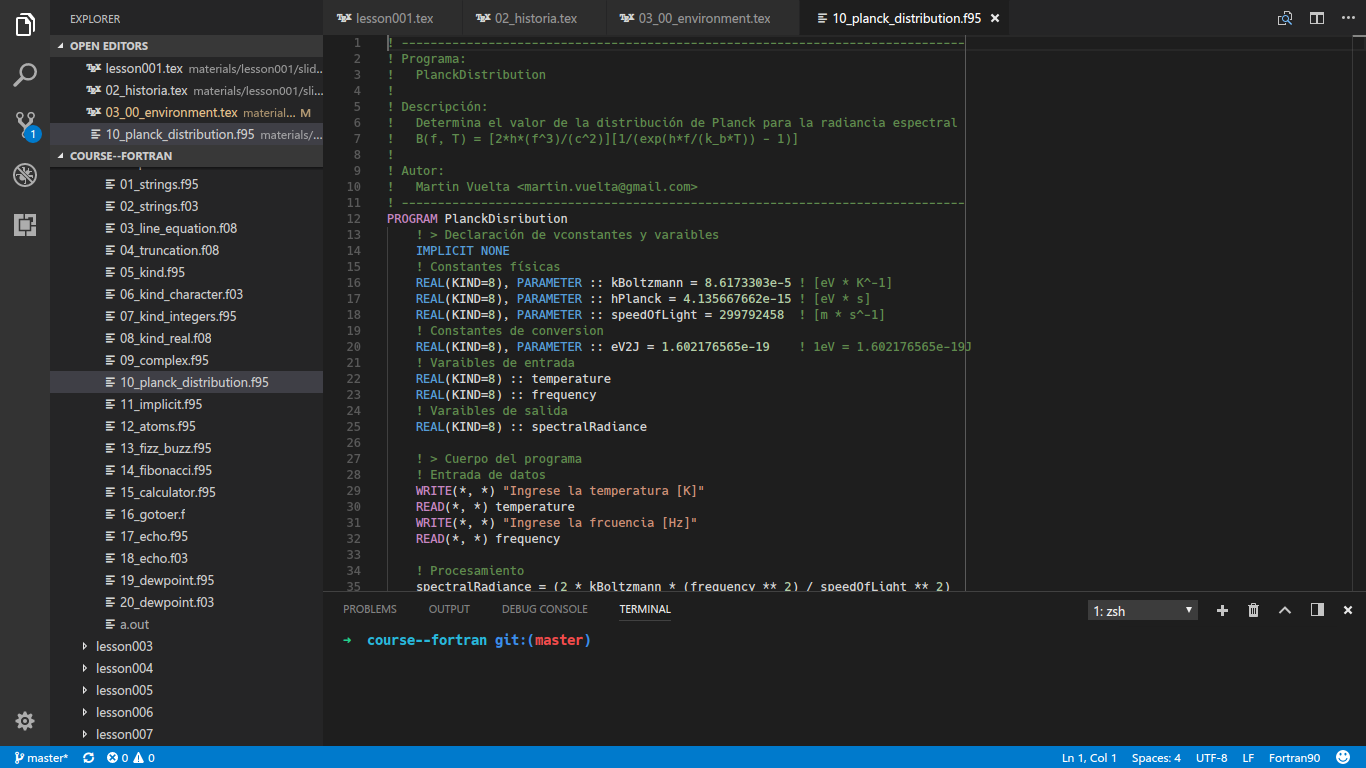
\includegraphics[width=1\textwidth]{./resources/IDE-VSCODE.png}
      \caption{Entorno de desarrollo VS Code}
  \end{figure}
\end{frame}

\begin{frame}[fragile]{Entorno de desarrollo}
  \textbf{Que tiene un entorno de desarrollo}
  \begin{itemize}[<+(1)->]
    \item Editor de código
    \item Compiladores o intérpretes
    \item Debugger
    \item Otras utilidades
  \end{itemize}
\end{frame}


\begin{frame}[fragile]{Entorno de desarrollo}
  \textbf{Editor de código}
  \begin{itemize}[<+(1)->]
    \item VS Code + Fortran Package [{\color{green-600}\faCheck}]
    \item Sublime Text
    \item Atom
    \item Vim
    \item Emacs
    \item ...
  \end{itemize}
\end{frame}
 

\begin{frame}[fragile]{Entorno de desarrollo}
  \textbf{Compilador}
  \begin{itemize}[<+(1)->]
    \item GFortran [{\color{green-600}\faCheck}]
    \item Intel
    \item IBM
    \item Oracle
    \item ...
  \end{itemize}
\end{frame}


\begin{frame}[fragile]{Entorno de desarrollo}
  \textbf{Debuggers}
  \begin{itemize}[<+(1)->]
    \item gdb [{\color{green-600}\faCheck}]
    \item idb
    \item ddd
    \item totalview
    \item ...
  \end{itemize}
\end{frame}

  %-----------------------------------------------------------------------------80
% CONTENT
%-----------------------------------------------------------------------------80
\subsection{Entorno de desarrollo en Linux}
\begin{frame}[fragile]{Instalación de editor de código}
  \textbf{VS Code en Ubuntu y derivados}
\end{frame}


\begin{frame}[fragile]{Instalación de editor de código}
  \textbf{VS Code en Fedora / CentOS}
\end{frame}


\begin{frame}[fragile]{Instalación de compilador y debuger}
  \textbf{Compilador y debugger en Ubuntu y derivados}
\end{frame}


\begin{frame}[fragile]{Instalación de compilador y debuger}
  \textbf{Compilador y debugger en Fedora / CentOS}
\end{frame}

  %-----------------------------------------------------------------------------80
% CONTENT
%-----------------------------------------------------------------------------80
\subsection{Entorno de desarrollo Windows}
\begin{frame}[fragile]{Instalación de editor de código}
  \textbf{VS Code}
  \begin{itemize}[<+(1)->]
  \item Descargar el instalador desde \url{https://code.visualstudio.com/download}
  \item adasd
  
 \end{itemize}
\end{frame}


\begin{frame}[fragile]{Instalación de compilador y debuger}
 \textbf{Instalación del compilador TDM-GCC}
 \begin{itemize}[<+(1)->]
  \item Descargar el paquete TDM-GCC según la versión de windows (32-64 bits) en \url{http://tdm-gcc.tdragon.net/}
  \item asdasd
 \end{itemize}
\end{frame}


\end{document}
